\documentclass{article}
\usepackage{graphicx}
\usepackage{alltt}
\usepackage{amsmath}
\usepackage{amsfonts}
\usepackage{bigstrut}
\usepackage{enumerate}
\usepackage{fancyhdr}
\usepackage[top=.75in, bottom=.95in, left=.75in, right=.75in]{geometry}
\usepackage{float}
\usepackage{lastpage}
\usepackage{tikz}
\usepackage[latin1]{inputenc}
\usepackage{color}
\usepackage{array}
\usepackage{longtable}
\usepackage{calc}
\usepackage{multirow}
\usepackage{hhline}
\usepackage{ifthen}
\usepackage{listings}
\usepackage{circuitikz}
\usepackage{caption}
\definecolor{mygreen}{rgb}{0,0.6,0}
\definecolor{mygray}{rgb}{0.5,0.5,0.5}
\definecolor{mymauve}{rgb}{0.58,0,0.82}
\lstset{ %
  backgroundcolor=\color{white},   % choose the background color; you must add \usepackage{color} or \usepackage{xcolor}; should come as last argument
  basicstyle=\normalsize,        % the size of the fonts that are used for the code
  breakatwhitespace=false,         % sets if automatic breaks should only happen at whitespace
  breaklines=true,                 % sets automatic line breaking
  captionpos=b,                    % sets the caption-position to bottom
  commentstyle=\color{mygreen},    % comment style
  deletekeywords={...},            % if you want to delete keywords from the given language
  escapeinside={\%*}{*)},          % if you want to add LaTeX within your code
  extendedchars=true,              % lets you use non-ASCII characters; for 8-bits encodings only, does not work with UTF-8
  frame=single,	                   % adds a frame around the code
  keepspaces=true,                 % keeps spaces in text, useful for keeping indentation of code (possibly needs columns=flexible)
  keywordstyle=\color{blue},       % keyword style
  language=python,                  % the language of the code
  morekeywords={*,...},            % if you want to add more keywords to the set
  numbers=left,                    % where to put the line-numbers; possible values are (none, left, right)
  numbersep=5pt,                   % how far the line-numbers are from the code
  numberstyle=\tiny\color{mygray}, % the style that is used for the line-numbers
  rulecolor=\color{black},         % if not set, the frame-color may be changed on line-breaks within not-black text (e.g. comments (green here))
  showspaces=false,                % show spaces everywhere adding particular underscores; it overrides 'showstringspaces'
  showstringspaces=false,          % underline spaces within strings only
  showtabs=false,                  % show tabs within strings adding particular underscores
  stepnumber=2,                    % the step between two line-numbers. If it's 1, each line will be numbered
  stringstyle=\color{mymauve},     % string literal style
  tabsize=2,	                   % sets default tabsize to 2 spaces
  title=\lstname                   % show the filename of files included with \lstinputlisting; also try caption instead of title
}
\floatstyle{boxed}
\floatstyle{plain}
\restylefloat{figure}
\pagestyle{fancy}
\fancyhead{}
\fancyfoot{}
\setlength{\headheight}{59.0pt}
\def\inputGnumericTable{}
\fancyhead[CO]{\textbf{Air Force Institute of Technology\\Department of Electrical and Computer Engineering\\
 Computer Communication Networks (CSCE-654) Project \#2\newline \newline Name: Micah Hayden}}
\lhead{\today}
\rhead{Page \thepage{} of \pageref{LastPage} }
\newlength\tindent
\setlength{\tindent}{\parindent}
\setlength{\parindent}{0pt}
\renewcommand{\indent}{\hspace*{\tindent}}
\begin{document}

%\begin{abstract}
%This is my abstract.
%\end{abstract}

\section*{Simulation Setup:}
I utilized the provided FIFO queue sample project as the starting point for my simulation.

\subsection*{Network Configuration}  
My "Tandem Satellite" network consisted of one generator, two FIFO queues/servers, a satellite node, and a sink node.  
The generator, queue, and sink nodes are all the same as given in the FIFO sample (and the same as Project \#1).  
I defined the satellite node as a simple node which handled any incoming message by forwarding it to the following node immediately.  
Due to the distance to the satellite, the simulation needed to account for the propagation delay.
\begin{align*}
& t_{prop} = \frac{d}{c} \hspace{2cm} d = 42,000km  \hspace{1cm} c = 299,792,458 \frac{m}{s} \\
& t_{prop} = \frac{4.2 \times 10^7 m}{299792458 \frac{m}{s}} \\
& \boxed{t_{prop} = 0.1401 s}
\end{align*}
The satellite node accounted for the propagation delay of communication with the satellite by using a channel delay on the links connecting the satellite to the two queues.
Figure \#\ref{diagram} shows this network setup. 

\begin{figure}[h!]
	\begin{center}
	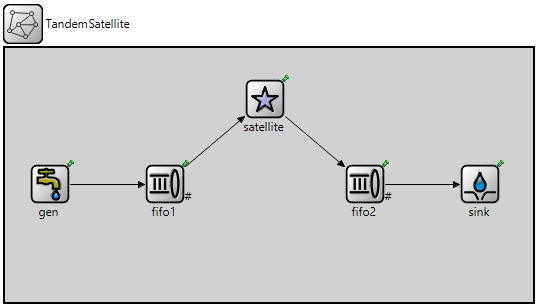
\includegraphics[scale=1.0]{Images/TandemSatellite.PNG}
	\vspace{-.25cm}
	\caption{Network diagram}
	\label{diagram}
	\end{center}
\end{figure}

When a packet arrives at the sink, it generates a packet delay data point as defined in Eq. \#\ref{delay}
\begin{equation}
	\label{delay}
	Packet \, Delay = time_{arrival} - time_{created}
\end{equation}

\newpage
\subsection*{Simulation Time:}  
Before determining a simulation run-time, I calculated $\lambda$, $\mu$, and $\rho$ from the mean service time and interarrival times specified.
Table \#\ref{Parameters} below.
\begin{table}[h!]
\centering
\begin{tabular}{|c|c|c|c|c|} \hline
\textbf{Case \#:} & \textbf{Interarrival Time (s)} & $\mathbf{\lambda}$ & $\mathbf{\mu}$ & $\mathbf{\rho}$ \\ \hline
1 & 1.00 & 1.00 & 2.00 & 0.50 \\ \hline
2 & 0.52 & 1.92 & 2.00 & 0.96 \\ \hline
3 & 0.50 & 2.00 & 2.00 & 1.00 \\ \hline 
\end{tabular}
\caption{Queue Parameters}
\label{Parameters}
\end{table}

Based on these parameters, Case \#3 should become unstable, given a long enough simulation.
I started by running the three cases for 1 hour each.  
However, when I plotted the data, the second case with $t_{IA}=0.52 \, seconds$ actually had a longer average system delay than the final case with $t_{IA}=0.50 \, seconds$, and similar average queue lengths.  
Based on this result, I decided that a longer simulation was needed.  
My final simulation run-time was 10 hours, which generated a result aligning with the expectation given the relationship between $\lambda$ and $\mu$.

\section*{Results \& Analysis:}

\subsection*{System Delay}

\subsubsection*{Expected Results}
Using $\lambda$ and $\mu$, and the calculated values for $\rho$, one can calculate the expected time in the system, $E[r]$; and the expected time in the queue $E[w]$, using the relationships below, derived from Little's Law.
\begin{align*}
E[r]_{system} = \frac{1}{\mu - \lambda} \hspace{0.15\textwidth} E[w]_{queue} = \frac{\rho}{\mu - \lambda} \\
\end{align*}

However, the above equations do not account for duplicate queues, or propagation delay.
Thus, the actual relationship for the tandem queue system requires some additional manipulation, shown below:
\begin{align*}
 E[r]_{actual} &= 2 \cdot E[r] + 2 \cdot t_{prop} \hspace{.15\textwidth} E[w]_{actual} = 2 \cdot E[w] \, \text{seconds}	\\
			   &=2 \cdot E[r] + 0.28 \, \text{seconds}  \\
\end{align*}

Table \#\ref{tab:expectDelay} shows these results for each of the three cases.
Case 3 has an infinite expectation because it is an unstable system with $\rho = 1$.
\begin{table}[h!]
\centering
\begin{tabular}{|c|c|c|} \hline
\textbf{Case \#} & \textbf{E[r]$_{actual}$} & \textbf{E[w]$_{actual}$} \\ \hline
1 & 2.28 & 1.00  \\ \hline
2 & 26.28 & 24.00 \\ \hline
3 & $\infty$ & $\infty$ \\ \hline 
\end{tabular}
\caption{Expected System and Queue Delay}
\label{tab:expectDelay}
\end{table}

\newpage
\subsubsection*{Simulation Results}
Figure \#\ref{DelayPlot} shows the system delay of each case.

\begin{figure}[h!]
	\begin{center}
	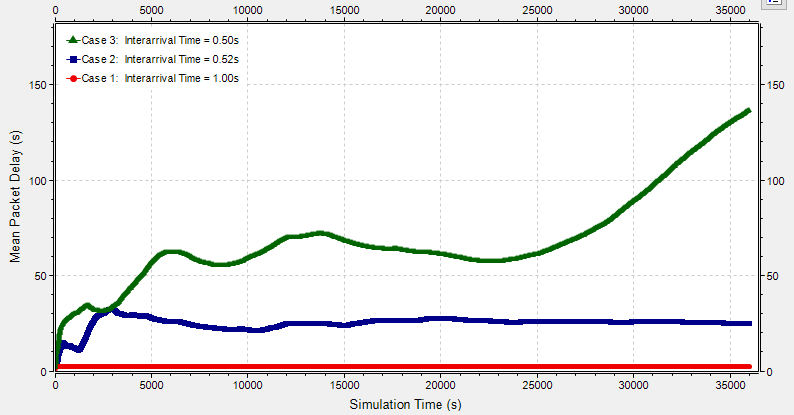
\includegraphics[scale=0.85]{Images/DelayPlot.PNG}
	\vspace{-.25cm}
	\caption{System Delay of varied interarrival times}
	\label{DelayPlot}
	\end{center}
\end{figure}

This simulation matched the expected system delays calculated previously, with averages of 2.24 seconds, 24.71 seconds, and 136.75 seconds, respectively for Cases 1-3.

\begin{table}[h!]
\centering
\begin{tabular}{|c|c|} \hline
\textbf{Case \#} & \textbf{Mean Packet Delay (s)} \\ \hline
1 & 2.24  \\ \hline
2 & 24.71 \\ \hline
3 & 136.75  \\ \hline 
\end{tabular}
\caption{Simulated Mean Packet Delay}
\label{tab:meanPacketDelay}
\end{table}


Case \#1 had a $1.8\%$ difference from the expected value, while Case \#2 had a $6.0\%$ difference.
Despite only having a difference of $0.02s$ in interarrival times, the average delay of Cases 2 and 3 were significantly different. 
The mean delay for Case \#3 was 136.75 seconds.  
This occurs because when $\rho = 1$, the system is unstable and the queue will grow to indefinitely.

\newpage
\subsection*{Queue Length \& Queue Time}

\subsubsection*{Expected Results}
Again using Little's Law, one can calculate the expected number in the queue $N_Q$.
Note, although there are two separate FIFO queues, they both have the same expected queue length and time.
\begin{align*}
N_Q = \frac{\rho^2}{1-\rho}
\end{align*}

\begin{table}[h!]
\centering
\begin{tabular}{|c|c|} \hline
\textbf{Case \#} & $N_Q$ \\ \hline
1 & 0.50  \\ \hline
2 & 23.04 \\ \hline
3 & $\infty$  \\ \hline 
\end{tabular}
\caption{Expected Queue Length}
\label{tab:expectQlen}
\end{table}

The expected queue time was detailed in the Expected Results for the System Delay
\subsubsection*{Simulation Results}
As shown in Tables 2 \& 3, the average queue lengths and queue times increased relative to the system delay.  
Case \#1 had a low number of packets in the queue because its arrival rate $\lambda_1 = 0.5 \cdot \mu$.

\begin{minipage}{0.5\textwidth}
	\centering
	\begin{tabular}{|c|c|c|c|} \hline
		\textbf{Module} & \textbf{Case \#} & \textbf{Mean (packets)} & \textbf{Std. Dev} \\ \hline
	 fifo1 & 1 & 1.51 & 1.53 \\ \hline
	 fifo2 & 1 & 1.46 & 1.46 \\ \hline
	 fifo1 & 2 & 22.95 & 22.35 \\ \hline
	 fifo2 & 2 & 25.20 & 22.68 \\ \hline
	 fifo1 & 3 & 111.81 & 82.53 \\ \hline
	 fifo2 & 3 & 165.06 & 206.42 \\ \hline
	\end{tabular}
	\captionof{table}{Queue Length }
	\label{qlen}
\end{minipage}  
\begin{minipage}{0.5\textwidth}
	\centering
	\begin{tabular}{|c|c|c|c|} \hline
		\textbf{Module} & \textbf{Case \#} & \textbf{Mean (s)} & \textbf{Std. Dev} \\ \hline
		fifo1 & 1 & 0.50 & 0.87 \\ \hline
		fifo2 & 1 & 0.47 & 0.82 \\ \hline
		fifo1 & 2 & 11.15 & 11.36 \\ \hline
		fifo2 & 2 & 12.27 & 11.46 \\ \hline
		fifo1 & 3 & 54.92 & 40.91 \\ \hline
		fifo2 & 3 & 80.52 & 101.61 \\ \hline
	\end{tabular}
	\captionof{table}{Queue Time}
	\label{qTime}
\end{minipage}

These results matched the expected results fairly well.
For Case 1, there was a mean queue length of 1.49, compared to an expected queue length of 0.5, so a 1 packet difference.
Case 2 had an average queue length of 24.08, compared to an expected queue length of 23.04.
Finally, Case 3 had an average queue length of 138.44.

For the queue time, one would expect the expected waiting time calculated in the system delay to equal the sum of the queue time in fifo1 and fifo2.
For Case 1, there was an average \textbf{total} queue time of 0.97 seconds, compared to 1.00 seconds.
Case 2 had an average total queue time of 23.42 seconds, compared to the expected queue time of 24.00 seconds.
Finally, Case 3 had an average total queue time of 135.44 seconds.

\subsection*{Propagation Delay}
One can see the propagation delay of the simulation by comparing the average lifetime to the sum of the queue times and service times.
\begin{align*}
\text{Prop Delay} = \text{Mean lifetime} - time_{fifo1} - time_{fifo2} - 2 \cdot \text{service time}
\end{align*}

In practice, the mean times produced the following calculated propagation delays:

\begin{table}[h!]
\centering
\begin{tabular}{|c|c|} \hline
\textbf{Case \#} & \textbf{Prop. Delay (s)} \\ \hline
1 & 0.27 \\ \hline
2 & 0.29 \\ \hline
3 & 0.31 \\ \hline
\end{tabular}
\caption{Calculated Propagation Delays}
\label{tab:calcPropDelay}
\end{table}


\section*{Conclusions}
This project demonstrated the long term effects of a queuing system for different values of $\rho$.  
When $\lambda$ is much less than $\mu$, the system is able to keep up, and produces minimal delays.  
As $\lambda$ approaches $\mu$, the queue will increase in length; however, as long as $\lambda < \mu$, the system will still be stable.
Once $\lambda = \mu$, the system becomes unstable, and will have a system delay and queue length that will grow indefinitely.

Another interesting outcome of this experiment was seeing the effects of the propagation delay.  
One would expect the two queues to have identical times in the long run; however, they were slightly different for all simulations.
Because of these variations, using the average queue times and average lifetime to calculate the propagation delay produced a slightly different value than the constant specified in the simulation, as shown in Table \#\ref{tab:calcPropDelay}.
This shows the inherent complexity of a system of queues, even when the queues have the same parameters for expected arrival rates and service rates.


\newpage
\section*{Appendix A:  Figures}

\begin{figure}[h!]
	\begin{center}
	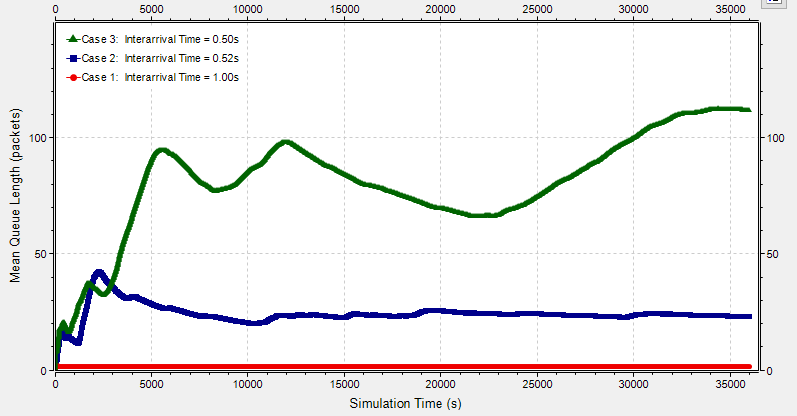
\includegraphics[scale=0.75]{Images/Fifo1_QueueLength.PNG}
	\vspace{-.25cm}
	\caption{Fifo1 Mean Queue Length}
	\label{fifo1_qlen}
	\end{center}
\end{figure}

\begin{figure}[h!]
	\begin{center}
	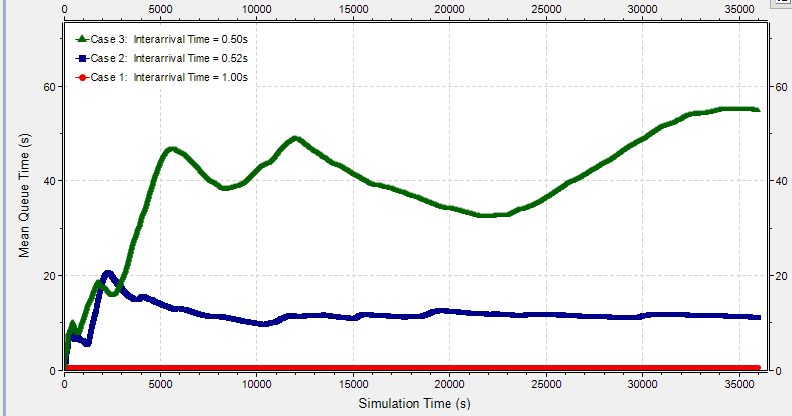
\includegraphics[scale=0.75]{Images/Fifo1_QueueTime.PNG}
	\vspace{-.25cm}
	\caption{Fifo1 Mean Queue Time}
	\label{fifo1_qtime}
	\end{center}
\end{figure}

\begin{figure}[h!]
	\begin{center}
	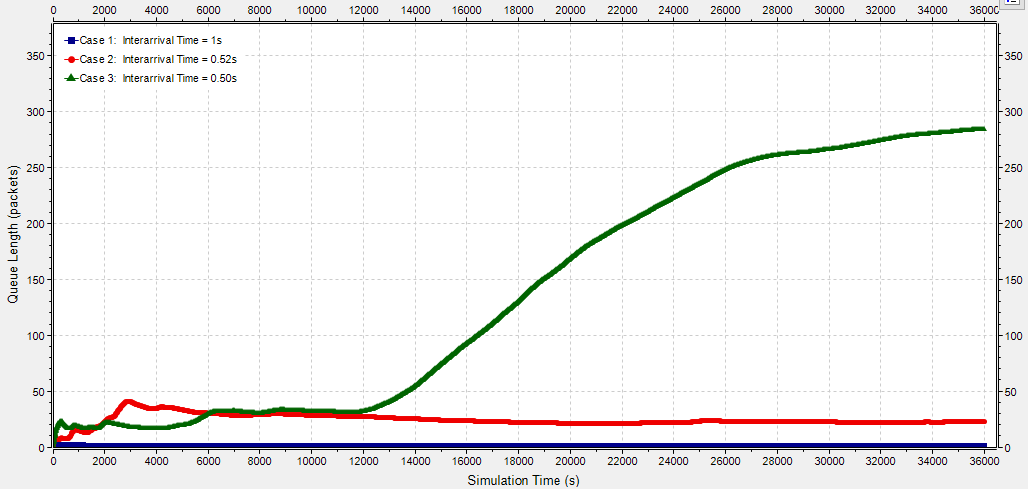
\includegraphics[scale=0.75]{Images/Fifo2_QueueLength.PNG}
	\vspace{-.25cm}
	\caption{Fifo2 Mean Queue Length}
	\label{fifo2_qlen}
	\end{center}
\end{figure}

\begin{figure}[h!]
	\begin{center}
	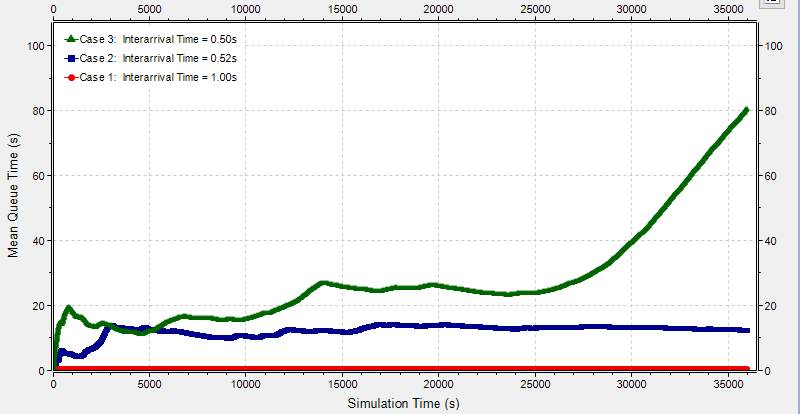
\includegraphics[scale=0.75]{Images/Fifo2_QueueTime.PNG}
	\vspace{-.25cm}
	\caption{Fifo2 Mean Queue Time}
	\label{fifo2_qtime}
	\end{center}
\end{figure}

\newpage
\clearpage
\section*{Appendix B:  Simulation Files}

\begin{figure}[h!]
\begin{lstlisting}
[General]
network = TandemSatellite
sim-time-limit = 10h
cpu-time-limit = 300s
#debug-on-errors = true
#record-eventlog = true

[Config TandemQueue]
**.gen.sendIaTime = exponential( ${m=1.0, 0.52, 0.50}s )
**.fifo*.serviceTime = exponential(0.5s)
**.satellite.propDelay = 0.1401s

[Config Tandem1]
description = "Arrival rate of 1s"
**.gen.sendIaTime = exponential(1s)
**.fifo*.serviceTime = exponential(0.5s)
**.satellite.propDelay = 0.1401s

[Config Tandem2]
description = "Arrival rate of 0.52s"
**.gen.sendIaTime = exponential(0.52 s)
**.fifo*.serviceTime = exponential(0.5s)
**.satellite.propDelay = 0.1401s

[Config Tandem3]
description = "Arrival rate of 0.5s"
**.gen.sendIaTime = exponential(0.5 s)
**.fifo*.serviceTime = exponential(0.5s)
**.satellite.propDelay = 0.1401s
\end{lstlisting}
\vspace{-1cm}
\caption*{Simulation Initialization File - omnetpp.ini}
\end{figure}

\newpage
\begin{figure}[h!]
\begin{lstlisting}
network TandemSatellite
{
    @display("bgb=528,254");
    submodules:
        gen: Source {
            parameters:
                @display("p=45,136");
        }
        fifo1: Fifo {
            parameters:
                @display("p=160,136");
        }
        fifo2: Fifo {
            parameters:
                @display("p=360,136");
        }
        satellite: Satellite {
            parameters:
                @display("p=260,51");
        }
        sink: Sink {
            parameters:
                @display("p=475,136");
        }
    connections:
        gen.out --> fifo1.in;
        fifo1.out --> {  delay = satellite.propDelay; } --> satellite.in;
        satellite.out --> {  delay = satellite.propDelay; } --> fifo2.in;
        fifo2.out --> sink.in;
}
\end{lstlisting}
\vspace{-1cm}
\caption*{Simulation Setup - Tandem\_Satellite.ned}
\end{figure}

\end{document}
